\section{Durchführung}
\label{sec:Durchführung}
Zu Beginn wird mit einem Voltmeter die Leerlaufspannung der Monozelle gemessen.
Der Eigenwiderstand des Voltmeters wird notiert.

\begin{figure}[H]
  \centering
  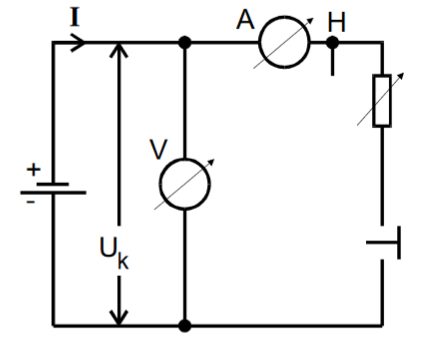
\includegraphics[height=5cm]{Schaltung.PNG}
  \caption{Schaltung zur Bestimmung des Innenwiderstandes.}
  \label{fig:Schaltung}
\end{figure}

Entsprechend Abbildung \ref{fig:Schaltung} wird die Monozelle nun in einen
Stromkreis integriert. Der eingebaute Widerstand (0-50\Omega) wird stückweise variiert und
die entsprechend gemessenen Werte von Stromstärke und Spannung abgelesen.

\begin{figure}[H]
  \centering
  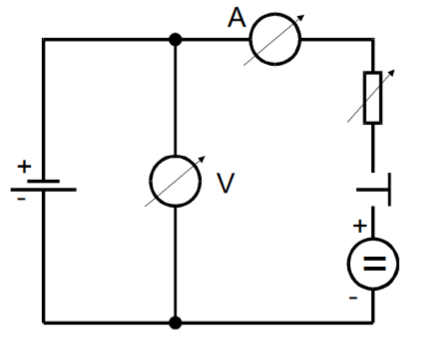
\includegraphics[height=5cm]{Schaltung1.PNG}
  \caption{Schaltung zur Bestimmung des Innenwiderstandes mit Gegenspannung.}
  \label{fig:Schaltung}
\end{figure}

Anschließend wird eine Gegenspannung wie in Abbildung \ref{fig:Schaltung1}
eingebunden. Die Messung von Strom und Spannung erfolgt analog.

Im letzten Teil des Versuchs wird dann wieder eine Schaltung wie in Abbildung
\ref{fig.Schaltung} verwendet. Jedoch wird als Spannungsquelle keine Gleichspannung,
sondern jeweils eine Rechteck- und eine Sinusspannung verwendet. Auch hier werden
Strom und Spannung auf die gleiche Weise gemessen, jedoch werden andere Widerstände
verwendet (Rechteckspannung: 20 - 250 \Omega, Sinusspannung: 0,1 - 5 k\Omega).
